\documentclass[preprint, 10pt]{elsarticle}

\newcommand{\mcaption}[2]{\caption{\small \em #1}\label{#2}}
\newcommand{\secref}[1]{\ref{#1}}

\usepackage{amsfonts}
\usepackage[fleqn,reqno]{amsmath}
\usepackage{amssymb}
\usepackage[titletoc]{appendix}
\usepackage{enumitem}
\usepackage{filecontents}
\usepackage[top=1.2in,bottom=1.2in,left=1in, right=1in]{geometry}
\usepackage{graphics}
\usepackage{lineno}
%\usepackage{showkeys} %To see the labels for now.  Will remove later
\usepackage{pgfplots}
\usepackage{tikz}
\usepackage{todonotes}

\usetikzlibrary{arrows}


%%%%%%  pdftex  %%%%%%%%%%%%%%%%%%%%%%%%%%%%%%%%%%%%%%%%%%%%%%%%%%%%%%
\usepackage[pagebackref=false,bookmarks=false]{hyperref} 

\hypersetup{
  bookmarksnumbered=true,
  bookmarksopen=false,
  hypertexnames=false,      
  breaklinks=true,          
  unicode=false,
  pdffitwindow=true,        
  pdfnewwindow=true,        
  colorlinks=true,         
  linkcolor=dblue,
  anchorcolor=red,
  citecolor=dorange,
  filecolor=magenta,
  urlcolor=dblue,
  pdfstartview = FitH,
  pdfkeywords = {},
  pdfcreator = {LaTeX with hyperref package}
}

\newcommand{\bd}{{\partial}}
\newcommand{\cc}{{\mathbf{c}}}
\newcommand{\DD}{{\mathcal{D}}}
\newcommand{\eeta}{{\boldsymbol\eta}}
\newcommand{\ff}{{\mathbf{f}}}
\newcommand{\grad}{{\nabla}}
\newcommand{\llambda}{{\boldsymbol\lambda}}
\newcommand{\nn}{{\mathbf{n}}}
\newcommand{\NN}{{\mathcal{N}}}
\newcommand{\pderiv}[2]{\frac{\partial #1}{\partial #2}}
\newcommand{\rr}{{\mathbf{r}}}
\newcommand{\RR}{{\mathbb{R}}}
\renewcommand{\ss}{{\mathbf{s}}}
\newcommand{\ssigma}{{\boldsymbol\sigma}}
\newcommand{\uu}{{\mathbf{u}}}
\newcommand{\UU}{{\mathbf{U}}}
\newcommand{\vv}{{\mathbf{v}}}
\newcommand{\xx}{{\mathbf{x}}}
\newcommand{\xxi}{{\boldsymbol{\xi}}}
\newcommand{\yy}{{\mathbf{y}}}

\begin{document}

\title{Methods paper for rigid bodies}

\author[Lukas]{Lukas Bystircky}
\author[Lukas]{Sachin Shanbhag}
\author[Bryan]{Bryan D.~Quaife}
\address[Lukas]{Department of Scientific Computing, Florida State University, Tallahassee, FL, 32306.}
\address[Bryan]{Department of Scientific Computing and Geophysical Fluid Dynamics Institute, Florida State University, Tallahassee, FL, 32306.}

\begin{abstract} 
We consider suspensions of rigid bodies in two dimensions \ldots
\end{abstract}

\begin{keyword}
  Stokes flow \sep Boundary integral method \sep Rigid body suspensions 
\end{keyword}

\maketitle





%%%%%%%%%%%%%%%%%%%%%%%%%%%%%%%%%%%%%%%%%%%%%%%%%%%%%%%%%%%%%%%%%%%%%%%
\section{Introduction\label{s:intro}}

\todo[inline]{Bryan will write this section}

This is a methods paper
\begin{itemize}
  \item Boundary integral equation formulation
  \item STIV
  \item FMM
  \item Near-singular integration
  \item Pressure and energy dissipation calculations
  \item Time integrator
\end{itemize}




%%%%%%%%%%%%%%%%%%%%%%%%%%%%%%%%%%%%%%%%%%%%%%%%%%%%%%%%%%%%%%%%%%%%%%%
\section{Formulation\label{s:formulation}} 



\subsection{Problem Formulation}

We consider a suspension of rigid particles flowing in a two dimensional
domain, $\Omega$.  The boundary of the domain, denoted by $\Gamma$, may
be bounded or unbounded, and may be multiply-connected.  We let
$\Gamma_k$, $1 \leq k \leq M$ be the connected components of $\Gamma$,
and if the geometry is bounded, the solid wall containing all other
solid walls is $\Gamma_0$.  The boundary of the suspended particles is
denoted by $\gamma_k$, $1 \leq k \leq N$, so that the fluid domain is
\begin{align*}
  \bd\Omega = \bigcup_{k=0}^M \Gamma_k \cup \bigcup_{k=1}^N \gamma_k,
\end{align*}
and $\Gamma_0$ is excluded if the domain is unbounded.  Since the
particles are rigid, we only track the center and angle of the suspended
particles will be written as $\cc_k$ and $\theta_k$, respectively, and
the translational and rotational velocities are written as $\uu_k^\tau$
and $\omega_k$, respectively.  Finally, each solid wall and rigid
particle will have a net force $\FF$ and net torque $L$ that it applies
to the fluid.  A schematic of the geometry is in
Figure~\ref{fig:geomSchematic}

%
%The fluid will be in a domain $\Omega$ with a boundary
%$\partial\Omega$. The boundary $\partial\Omega$ is the union of the
%surfaces of $N$ suspended particles each with a boundary $\gamma_k$,
%$1\leq k \leq N$, the surfaces of $M$ solid walls each with boundary,
%$\Gamma_\ell$, $1\leq\ell\leq M$ and optionally a containing wall
%denoted $\Gamma_0$. The suspended particles are all rigid and at each
%time step we will solve for their translational velocity
%$\mathbf{u}^{\tau}_k$ and angular velocity $\omega_k$, allowing us to
%update their centers and orientations, $\mathbf{c}_k$ and $\theta_k$
%respectively. Particles and interior walls will be undergoing a net
%force $\mathbf{F}_{k/\ell}$  and torque $L_{k/\ell}$. 

\begin{figure}[!h]
\begin{center}
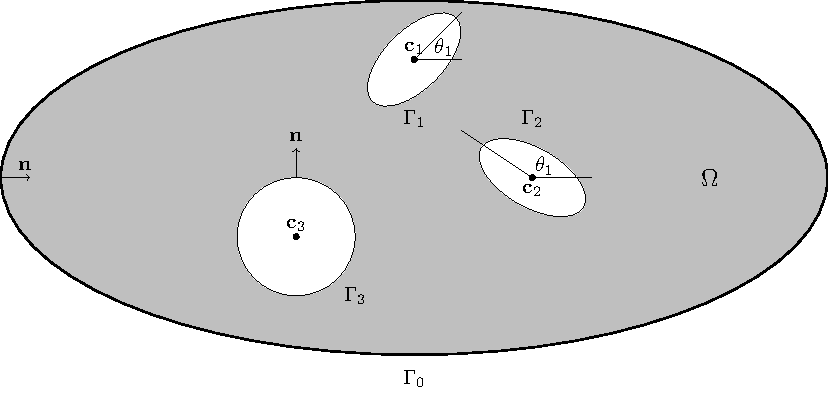
\includegraphics{figures/multiply_connected.pdf}
\end{center}
\caption{\label{fig:geomSchematic}Sketch of a possible domain $\Omega$.
  $\gamma_1$ and $\gamma_2$ enclose particles, while $\Gamma_1$ is a
  solid wall. The outer boundary $\Gamma_0$ need not be present.  The
  vector $\mathbf{n}$ is the unit normal vector pointing into the fluid
  domain.}
\end{figure}

\subsection{Governing Equations}\label{sec:governing}
At the continuum level the motion of a fluid is described by the
incompressible Navier-Stokes equations with dimensionless Reynolds
number
\begin{align*}
  \Re = \frac{UL}{\nu}
\end{align*},
where $U$ is a characteristic speed, $L$ is a characteristic lengths
scale, and $\nu$ is the kinematic fluid viscosity.  We are interested in
small particles and slow velocities which renders the Reynolds number
small $\Re \ll 1$.  Therefore, the fluid is governed by the
incompressible Stokes equations
\begin{subequations}\label{eq:stokes}
\begin{align}
  -\mu\Delta \mathbf{u} + \nabla p &= \mathbf{0} \text{ in }\Omega,\\	  
  \nabla\cdot\mathbf{u} &= 0 \text{ in }\Omega,
\end{align}
\end{subequations}
where $\mu$ is the viscosity, $\mathbf{u}(\mathbf{x})$ is the velocity,
and $p(\mathbf{x})$ is the pressure.  The boundary conditions on the
solid walls will be imposed, so the velocity satisfies the Dirichlet
boundary condition
\begin{align}
  \label{eq:boundary_condition}
  \mathbf{u} = \mathbf{u}_b, \quad \xx \in 
    \bigcup\limits_{k=0}^M \Gamma_\ell,
\end{align}
subject to the constraint 
\begin{align}
  \label{eq:compatibility}
  \int_{\bigcup\limits_{\ell=0}^M\Gamma_\ell} \uu_b\cdot\nn ds = 0.
\end{align}
On the particles we will assume no-slip boundary conditions, meaning the
velocity at any point on the surface of a particle matches the velocity
of the fluid.  Since the particles are rigid this can be expressed as,
\begin{align*}
  \uu = \uu^\tau_k + \omega(\xx-\cc_k)^\perp, \quad \xx \in \gamma_k.
\end{align*}



%%%%%%%%%%%%%%%%%%%%%%%%%%%%%%%%%%%%%%%%%%%%%%%%%%%%%%%%%%%%%%%%%%%%%%%%%%%%%%%
\subsection{Boundary Integral Equation Representation}
Since we are interested in solving a linear PDE, an integral equation
formulation is possible.  Moreover, a {\em boundary integral equation}
(BIE) formulation is possible.  This will have the advantage of a dimension
reduction in the number of unknowns while obtaining spectral accuracy,
and the resulting linear system will be solved with optimal complexity
by using a fast summation method.  A further discussion of the
advantages of a BIE formulation for the incompressible Stokes equations
can be found in Karrila and Kim~\cite{Karrila1989}.

As discussed in section \ref{sec:governing}, the governing equations for this problem are the incompressible Stokes equations. There are many ways to solve these equations, here we will use \textit{boundary integral equations} (BIEs). For the Stokes equations BIEs have many advantages, a discussion of which can be found in \cite{Karrila1989}. 

We our governing equations for a bounded geometry and then mention the
slight modification that must be made for unbounded geometries.  The
solution of the incompressible Stokes equations~\eqref{eq:stokes} at a
point $\xx \in \Omega$ can be expressed as the double layer
potential~\cite{Ladyzhenskaya1963, Pozrikidis1992}
\begin{align}
  \label{eq:dlp}
  \uu(\xx) = \DD[\eeta](\xx) = \frac{1}{\pi}\int_{\bd\Omega}
  \frac{\rr\cdot\mathbf{n}}{\rho^2}\frac{\rr \otimes \rr}{\rho^2}
  \eeta(\yy) ds_{\yy}, \quad \xx \in \Omega
\end{align}
where $\eeta$ is an unknown density function defined  on $\bd\Omega$,
$\rr = \xx - \yy$ and $\rho=|\rr|$.  The double layer potential by
itself cannot represent all possible flow fields. In particular it
cannot represent flows around surfaces undergoing a net force or torque.
Following \cite{Power1987, Power1993} for surfaces undergoing an
arbitrary net force $\mathbf{F}$ and net torque $L$ we complete the
double layer potential as,
\begin{align*}
  \uu(\xx) = \DD[\eeta](\xx) + \sum_{i=1}^{N+M} 
    \left(\mathbf{S}(\xx,\cc_i)\FF_i + \mathbf{R}(\xx,\cc_i)L_i\right),
\end{align*}
where the Stokeslet $\mathbf{S}(\mathbf{x},\mathbf{y})$ and rotlet $\mathbf{R}(\mathbf{x},\mathbf{y})$ are given by
\begin{align*}
  \mathbf{S}(\xx,\yy) = \frac{\rr \otimes \rr}{\rho^2} - 
  \log\rho\mathbf{I}, \qquad 
  \mathbf{R}(\xx,\yy) = \frac{\rr^\perp}{\rho^2}.
\end{align*}

To set up a system to solve we can take the limit of \eqref{eq:dlp} as we approach $\partial\Omega$ and match it to the boundary condition \eqref{eq:boundary_condition}. The double layer potential is not continuous when we cross the boundary and has a limiting value of $-\pmb{\eta}/2$. This leads to the second kind Fredholm equation,
\begin{equation}\label{eq:vel_walls} -\frac{1}{2}\pmb{\eta}(\mathbf{x}) + \mathcal{D}[\pmb{\eta}](\mathbf{x}) + \sum\limits_{i=1}^{N+M} \left(\mathbf{S}(\mathbf{x},\mathbf{c}_i)\mathbf{F}_i + \mathbf{R}(\mathbf{x},\mathbf{c}_i)L_i\right) = \mathbf{u}_b - \mathbf{u}_\infty.\end{equation}

On solid walls we will prescribe the velocity $\mathbf{u}_b$ and solve for the net force and torque on each wall. This is called the \textit{resistance problem}. For particles on the other hand we will prescribe the net force and torque on each particle and solve for the velocity $\mathbf{u}_b$. This is known as the \textit{mobility problem}. We will use the fact that the particles are rigid to decompose $\mathbf{u}_b$ into a translational and rotational component,
\[ \mathbf{u}_b = \mathbf{u}^\tau + \omega(\mathbf{x}-\mathbf{c})^\perp.\]
This lets us set up an equation to solve for the velocity on the surface of particle $k$,
\begin{equation}\label{eq:vel_particles} -\frac{1}{2}\pmb{\eta}(\mathbf{x}) + \mathcal{D}[\pmb{\eta}](\mathbf{x}) - \mathbf{u}^\tau_k - \omega(\mathbf{x}-\mathbf{c}_k)^\perp =  -\sum\limits_{i=1}^{N+M} \left(\mathbf{S}(\mathbf{x},\mathbf{c}_i)\mathbf{F}_i + \mathbf{R}(\mathbf{x},\mathbf{c}_i)L_i\right) - \mathbf{u}_\infty.\end{equation}

For the both the resistance and mobility problem we have more unknowns than equations. In particular, we have to solve for two components of $\pmb{\eta}$ and either 
\begin{enumerate}[label=(\alph*)]
	\item two components of net force and a net torque for each solid wall $\rightarrow$ an additional $3M$ unknowns
	\item two components of translational velocity and an angular velocity of each particle $\rightarrow$ an additional $3N$ unknowns
\end{enumerate}

To close these systems we will follow \cite{Power1993} and relate $\pmb{\eta}$ to the net force and torque on each particle or wall. In particular for $1\leq i \leq N+M$,
\begin{subequations}\label{eq:closure}
\begin{align}
	&\int_{\Gamma_i} \pmb{\eta}~\text{d}s = \mathbf{F}_i,\\
	&\int_{\Gamma_i} \pmb{\eta}\cdot (\mathbf{x} - \mathbf{c})^\perp~\text{d}s = L_i.
\end{align} 
\end{subequations}

Combining \eqref{eq:vel_walls}, \eqref{eq:vel_particles} and \eqref{eq:closure} we can write our problem in the compact notation,
\begin{equation}\label{eq:stokes_unbounded} \begin{bmatrix} -\frac{1}{2} + \mathcal{D} & 1 & (\mathbf{x}-\mathbf{c})^\perp & \mathcal{S} & \mathcal{R}\\
		\int \cdot~ \text{d}s & 0 & 0 & 0 & 0\\
		\int\cdot(\mathbf{x}-\mathbf{c})^\perp~\text{d}s & 0 & 0 & 0 & 0\\
		\int \cdot~ \text{d}s & 0 & 0 & - 1 & 0\\
		\int\cdot(\mathbf{x}-\mathbf{c})^\perp~\text{d}s & 0 & 0 & 0 & -1\end{bmatrix}
\begin{bmatrix}
	\pmb{\eta}\\\mathbf{u}^\tau \\ \pmb{\omega} \\ \mathbf{F}_w \\\mathbf{ L}_w
\end{bmatrix}
=
\begin{bmatrix}
	-\mathbf{u}_{\infty} - \mathcal{S}\mathbf{F}_p - \mathcal{R}\mathbf{L}_p\\
	\mathbf{F}_p\\
	\mathbf{L}_p\\
	0\\
	0
\end{bmatrix}
\end{equation}

\subsubsection{Bounded Domains}

Bounded domains lead to a similar system, however it must be modified slightly. For fluid inside a container the double layer potential has a rank one null space \cite{Ladyzhenskaya1963}. Following \cite{Power1993} this null space can be removed by adding an operator that is active only over the enclosing boundary $\Gamma_0$,
\[ \mathcal{N}_0[\pmb{\eta}](\mathbf{x}) = \delta_{i0} \int_{\Gamma_i}\mathbf{n}(\mathbf{x})\otimes\mathbf{n}(\mathbf{y})~\text{d}s(\mathbf{y}).\]
The compatibility condition \eqref{eq:compatibility} ensures that this term evaluates to 0. Adding $\mathcal{N}_0$ to \eqref{eq:stokes_unbounded} and removing the background flow leads to the linear system,
\begin{equation}\label{eq:stokes_bounded} \begin{bmatrix} -\frac{1}{2} + \mathcal{D} + \mathcal{N}_0 & 1 & (\mathbf{x}-\mathbf{c})^\perp & \mathcal{S} & \mathcal{R}\\
		\int \cdot~ \text{d}s & 0 & 0 & 0 & 0\\
		\int\cdot(\mathbf{x}-\mathbf{c})^\perp~\text{d}s & 0 & 0 & 0 & 0\\
		\int \cdot~ \text{d}s & 0 & 0 & - 1 & 0\\
		\int\cdot(\mathbf{x}-\mathbf{c})^\perp~\text{d}s & 0 & 0 & 0 & -1\end{bmatrix}
\begin{bmatrix}
	\pmb{\eta}\\\mathbf{u}^\tau \\ \pmb{\omega} \\ \mathbf{F}_w \\\mathbf{ L}_w
\end{bmatrix}
=
\begin{bmatrix}
	 - \mathcal{S}\mathbf{F}_p - \mathcal{R}\mathbf{L}_p\\
	\mathbf{F}_p\\
	\mathbf{L}_p\\
	0\\
	0
\end{bmatrix}
\end{equation}



%%%%%%%%%%%%%%%%%%%%%%%%%%%%%%%%%%%%%%%%%%%%%%%%%%%%%%%%%%%%%%%%%%%%%%%%%%%%%%%
\subsection{Repulsion Forces}

\begin{figure}[!h]\label{fig:collision_sketch}
\begin{center}
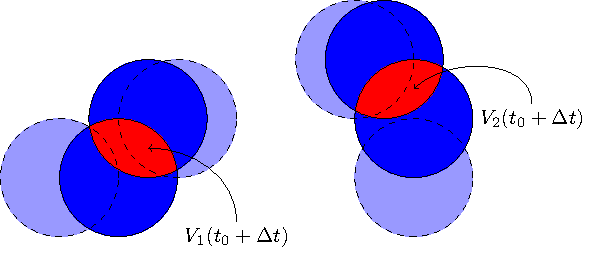
\includegraphics{figures/collisions.pdf}
\end{center}
\caption{Sketch of potential collisions.}
\end{figure}
It is well known that the exact solutions of the Stokes equations prohibit contact between particles in finite time due to lubrication forces. In theory therefore if we solve the Stokes equations accurately enough contact will be avoided. Achieving this level of accuracy requires a prohibitively fine mesh or small time step size, in particular for dense suspensions. In order to keep computational costs reasonable we must turn to alternative approaches. 

One such approach is to introduce an artificial repulsion force. There are many possible choices for the type of force. One possibility is a Leonard-Jones type force that grows exponentially as two particles become close together\todo{Need citations}. This has been shown to work for dense suspensions, however the resulting ODEs become very stiff as the separation between particles decreases, thus requiring smaller time steps. In addition this type of force does guarantee no collisions. If the time step is too large collisions can still occur. An alternative approach is to choose the forces in such a way as to explicitly guarantee each time step is collision free. 

The main algorithm will proceed as follows. At each time step $t^n$ the Stokes equations are solved and the particles are advanced to a candidate configuration at $t^{n+1}$. At this point we can check for collisions. If no collisions are found, the candidate configuration is accepted, otherwise it is rejected and we resolve the Stokes equations at $t^n$ with an artificial repulsion force, adjusting this force as necessary until the candidate configuration at time $t^{n+1}$ is collision free and can be accepted. The remainder of this section is dedicated to describing how this artificial repulsion force is computed. 


%%%%%%%%%%%%%%%%%%%%%%%%%%%%%%%%%%%%%%%%%%%%%%%%%%%%%%%%%%%%%%%%%%%%%%%%%%%%%%%
\subsection{Repulsion Forces}

\begin{figure}[!h]\label{fig:collision_sketch}
\begin{center}
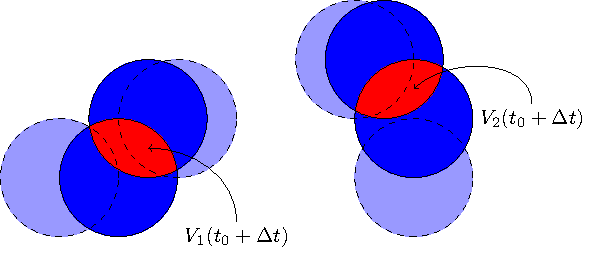
\includegraphics{figures/collisions.pdf}
\end{center}
\caption{Sketch of potential collisions.}
\end{figure}
It is well known that the exact solutions of the Stokes equations prohibit contact between particles in finite time due to lubrication forces. In theory therefore if we solve the Stokes equations accurately enough contact will be avoided. Achieving this level of accuracy requires a prohibitively fine mesh or small time step size, in particular for dense suspensions. In order to keep computational costs reasonable we must turn to alternative approaches. 

One such approach is to introduce an artificial repulsion force. There are many possible choices for the type of force. One possibility is a Leonard-Jones type force that grows exponentially as two particles become close together\todo{Need citations}. This has been shown to work for dense suspensions, however the resulting ODEs become very stiff as the separation between particles decreases, thus requiring smaller time steps. In addition this type of force does guarantee no collisions. If the time step is too large collisions can still occur. An alternative approach is to choose the forces in such a way as to explicitly guarantee each time step is collision free. 

The main algorithm will proceed as follows. At each time step $t^n$ the Stokes equations are solved and the particles are advanced to a candidate configuration at $t^{n+1}$. At this point we can check for collisions. If no collisions are found, the candidate configuration is accepted, otherwise it is rejected and we resolve the Stokes equations at $t^n$ with an artificial repulsion force, adjusting this force as necessary until the candidate configuration at time $t^{n+1}$ is collision free and can be accepted. The remainder of this section is dedicated to describing how this artificial repulsion force is computed. 



\subsection{Contact definition}

Before any discussion of resolving collisions we must define a metric that measures collisions. This metric tracks all pairwise collisions. If an entry of $\mathbf{V}(t)$ is less than 0 at a time $t$, then a collision has occurred and a repulsion force must be added. There are several possible choices for $\mathbf{V}(t)$, the simplest being a signed distance between all points on all particles. We use the concept of \textit{Space-Time Interference Volumes} (STIV) introduced by Harmon et al.~\cite{Harmon2011} and adapted for suspension modeling by Lu et al.~\cite{Lu2017}. 

Given a particle configuration $S(t)$ for which $S(t_0)$ is collision-free, for each point $\mathbf{X}(s,t)$ on $S(t)$ we define $\tau_I(s)$, $t_0 < \tau_I \leq t$ to be the first instance for which $\mathbf{X}$ comes into contact with a different point on $S(t)$. The STIV for the time interval $[t_0, t]$ is 
\[ V(S, t) = -\int_{S(t_0)}\int_{\tau_I(s)}^t \sqrt{\epsilon^2 + (\mathbf{u}(s, \tau)\cdot\mathbf{n}(s,\tau))^2}~\text{d}\tau\text{d}s,\]
where the constant $\epsilon$ is a smoothing parameter. The time integral in this expression ensures that no contact is missed even if one particle passes completely through another (or through a solid wall) in a single time step. This allows us to take large time steps and not be worried about missing collisions. $\mathbf{V}(S,t)$ can be interpreted as the area of the surface with coordinate $(\mathbf{X}(s,\tau),\epsilon\tau)$ for all $(s,\tau)$ such that $\tau_I(s)\leq t$. 

In \cite{Lu2017} an infinitesimal version of the STIV is derived. Starting from a collision-free configuration at $t_0$, for a fixed $\tau$ the set of points $s$ such that $\tau_I(s)\leq \tau$ is the contact area. This area is a set of boundary segments. For one such segment we can let $s_1(\tau)$ and $s_2(\tau)$ be the extents of contact at time $\tau$. 

\[ \mathbf{V}(\mathbf{u},t) = -\int_{s_1(t)}^{s_2(t)} \sqrt{\epsilon^2 + (\mathbf{u}(s,t)\cdot\mathbf{n}(s,t))^2}\text{d}s + \epsilon,\]
along with the variation, 
\[ \text{d}_{\mathbf{u}}V[\delta\mathbf{u}] = -\int_{s_1(t)}^{s_2(t)}\frac{(\mathbf{n}\cdot\mathbf{u})(\mathbf{n}\cdot\delta\mathbf{u})}{\sqrt{\epsilon^2 + (\mathbf{u}\cdot\mathbf{n})^2}}\text{d}s.\]




\subsection{Variational Formulation}

The incompressible Stokes equations can be can be restated as a minimization problem. Consider the functional,
\[ \mathcal{J}(\mathbf{u}) = \int_{\Omega} \nabla\mathbf{u}:\nabla\mathbf{u} - 2\mathbf{f}\cdot\mathbf{u} ~\text{d}\Omega,\]
and the associated constrained minimization problem,
\[ \min \mathcal{J}(\mathbf{u}) ~:~ \nabla\cdot\mathbf{u} = 0 \text{ in }\Omega.\]
Introducing $p$, a Lagrange multiplier for the incompressibility condition, we can construct a Lagrangian for this system,
\begin{equation}\label{eq:lagrangian} \mathcal{L}(\mathbf{u},p) = \mathcal{J}(\mathbf{u}) - \int_{\Omega} 2p\nabla\cdot\mathbf{u}~\text{d}\Omega.\end{equation}
First order optimality (KKT) conditions for $\mathcal{L}(\mathbf{u},p)$ recover the incompressible Stokes equations. For our problem, in addition to the incompressibility condition, we wish to enforce the constraint that the solution $\mathbf{u}$ at a time $t_0$ should not introduce collisions at time $t_0+\Delta t$, in other words $\mathbf{V}(t_0 + \Delta t) \geq \mathbf{0}$.
This constraint can be incorporated in the Lagrangian \eqref{eq:lagrangian} with the introduction of a Lagrange multiplier $\pmb{\lambda}$ with one component for each possible collision volume,
\begin{equation}\label{eq:lagrangian2} \tilde{\mathcal{L}}(\mathbf{u},p,\lambda) = \mathcal{L}(\mathbf{u},p) + \pmb{\lambda} \cdot \mathbf{V}(t_0+\Delta t).\end{equation}
First order optimality for \eqref{eq:lagrangian2} yields the Stokes equations with a modified forcing function,
\begin{equation}\label{eq:stokes_mod}-\Delta \mathbf{u} + \nabla p = \mathbf{f} + \int_{\Omega} \text{d}_{\mathbf{u}} \mathbf{V}^T\pmb{\lambda} ~\text{d}\Omega,\end{equation}
subject to the constraints
\[ \nabla\cdot\mathbf{u}  =0, ~\mathbf{V}(t_0 + \Delta t) \geq 0,~\pmb{\lambda} \geq 0, ~ \pmb{\lambda}\cdot\mathbf{V}(t_0+\Delta t) = 0.	\]

The constraints on $\mathbf{V}$ and $\pmb{\lambda}$ can be combined into a single constaint,
\begin{equation}\label{eq:ncp_constraint} \mathbf{V}(t_0 + \Delta t)\geq \mathbf{0} \perp \pmb{\lambda}\geq \mathbf{0}.\end{equation}


\subsection{Incorporating Repulsion Forces}

The addition of a forcing term to the right hand side of the Stokes equations would normally lead to a volume integral. However, in this case since $\text{d}_{\mathbf{u}} V$ can be non-zero only on the boundary, we can capture the repulsion force by adding a net force and torque to each particle or wall as needed. The net force $\mathbf{F}^k_p$ and torque $L^k_p$ are given by,
\[ \mathbf{F}^k_p = \int_{\Gamma_k} \text{d}_\mathbf{u}V^T\pmb{\lambda}~\text{d}s, \qquad L_p^k = \int_{\Gamma_k}  \text{d}_\mathbf{u}V^T\pmb{\lambda}\cdot(\mathbf{x}-\mathbf{c}_k)^\perp~\text{d}s.\]

\subsection{Complementary Problem}

To compute the repulsion forces we must first compute $\pmb{\lambda}$ for each time step such that \eqref{eq:ncp_constraint} is satisfied.
Consider particles suspended in a fluid in an amient flow $\mathbf{u}_\infty$. This flow can be an imposed background flow or come from solid walls. In the later case this velocity field is computed by solving the appropriate resistance problem. In either case this flow can be expressed as the sum of a translational component $\mathbf{u}_{\infty}^\tau$, a rotatial compoment $\omega_{\infty}$ and a strain component $\mathbf{e}_{\infty}$,
\[ \mathbf{u}_{\infty}(\mathbf{x}) =   \mathbf{u}_{\infty}^\tau + \omega_\infty\times \mathbf{x} + \mathbf{e}_\infty \cdot\mathbf{x}.\]
The translational and rotational velocity as well as the density function of a collection of particles can be computed from the force, torque and strain rate\cite{Karrila1991},
\begin{equation}\label{eq:mobility} \begin{bmatrix} \mathbf{u}_\infty^\tau - \mathbf{u}_\tau\\ \omega^\infty - \omega \\\pmb{\eta}\end{bmatrix} = \mathcal{M}\begin{bmatrix}\mathbf{F}\\\mathbf{L}\\\mathbf{e}_\infty\end{bmatrix},\end{equation}
where $\mathcal{M}$ is the \textit{mobility tensor} and depends only on the particle configuration $\mathbf{q}^0$. at some time $t^0$ Assuming the only force and torques acting on particles arises from repulsion forces, we can decompose \eqref{eq:mobility} as,
\[ \begin{bmatrix} \mathbf{u}_\infty^\tau - \mathbf{u}_\tau\\ \omega^\infty - \omega \\\pmb{\eta}\end{bmatrix} = \mathcal{M}\begin{bmatrix}\mathbf{0}\\\mathbf{0}\\\mathbf{e}_\infty\end{bmatrix} + \mathcal{M}\begin{bmatrix}\mathbf{F}_c\\\mathbf{L}_c\\\mathbf{0}\end{bmatrix}.\]

Once we solve for $\mathbf{u}_\tau$ and $\omega$ we can update the positions and angles of each particle using an explict Euler step. With an abuse of notation, this lets us express a candidate configuration $\mathbf{q}^{1}$ as,
\[ \mathbf{q}^{1} = \mathbf{q}^n +  \Delta t\left(\mathcal{M}\begin{bmatrix}\mathbf{0}\\\mathbf{0}\\\mathbf{e}_\infty\end{bmatrix} + \mathcal{M}\begin{bmatrix}\mathbf{F}_c\\\mathbf{L}_c\\\mathbf{0}\end{bmatrix}\right).\]

This candidate configuration must satifsy the constraint \eqref{eq:ncp_constraint}, which we will rewrite to show the dependence of $\mathbf{V}$ on both $\mathbf{q}^0$ and $\mathbf{q}^{1}$,
\begin{equation}\label{eq:ncp_new}\mathbf{V}(\mathbf{q}^0,\mathbf{q}^{1})\geq \mathbf{0}\perp \pmb{\lambda}^n\geq \mathbf{0} \Rightarrow  \mathbf{V}\left(\mathbf{q}^0, \mathbf{q}^0 +  \Delta t\left(\mathcal{M}\begin{bmatrix}\mathbf{0}\\\mathbf{0}\\\mathbf{e}_\infty\end{bmatrix} + \mathcal{M}\begin{bmatrix}\mathbf{F}_c\\\mathbf{L}_c\\\mathbf{0}\end{bmatrix}\right)\right) \geq \mathbf{0} \perp\pmb{\lambda}\geq \mathbf{0} .\end{equation}

This is a nonlinear complementary problem (NCP). We can see this by explicitly including the dependence of $\mathbf{V}$ on $\pmb{\lambda}$,
\[\mathbf{V}\left(\mathbf{q}^0, \mathbf{q}^0 +  \Delta t\left(\mathcal{M}\begin{bmatrix}\mathbf{0}\\\mathbf{0}\\\mathbf{e}_\infty\end{bmatrix} + \mathcal{M}\begin{bmatrix} \int_{\Gamma_k} \text{d}_\mathbf{u}\mathbf{V}^T\pmb{\lambda}~\text{d}s\\ \int_{\Gamma_k}  \text{d}_\mathbf{u}\mathbf{V}^T\pmb{\lambda}\cdot(\mathbf{x}-\mathbf{c}_k)^\perp~\text{d}s \\\mathbf{0}\end{bmatrix}\right)\right) \geq \mathbf{0} \perp\pmb{\lambda}\geq \mathbf{0} .\]

A first order linearization of this NCP turns it into a sequence of linear complementary problems (LCP). Starting from an initial guess for $\pmb{\lambda}$, $\pmb{\lambda}^0$ the following sequence should converge to the solution of \eqref{eq:ncp_new}:
\begin{equation}\label{eq:lcp}\begin{aligned}
\mathbf{V}\biggl(\mathbf{q}^0 + \Delta t\biggl(\mathcal{M}\begin{bmatrix}\mathbf{0}\\\mathbf{0}\\\mathbf{e}_\infty\end{bmatrix} &+ \mathcal{M}\begin{bmatrix} \int_{\Gamma_k} \text{d}_\mathbf{u}\mathbf{V}^T\pmb{\lambda}^\ell~\text{d}s\\ \int_{\Gamma_k}  \text{d}_\mathbf{u}\mathbf{V}^T\pmb{\lambda}^\ell\cdot(\mathbf{x}-\mathbf{c}_k)^\perp~\text{d}s \\\mathbf{0}\end{bmatrix}\biggr)\biggr) \\
&+ \Delta t \mathcal{M}\begin{bmatrix}\int_{\Gamma_k} \text{d}_\mathbf{u}\mathbf{V}^T\pmb{\lambda}^{\ell+1}~\text{d}s\\ \int_{\Gamma_k}  \text{d}_\mathbf{u}\mathbf{V}^T\pmb{\lambda}^{\ell+1}\cdot(\mathbf{x}-\mathbf{c}_k)^\perp~\text{d}s \\\mathbf{0}\end{bmatrix}\frac{\partial\mathbf{V}}{\partial \mathbf{q}^1} \geq \mathbf{0} \perp \pmb{\lambda}^{\ell+1} \geq \mathbf{0}.\end{aligned}\end{equation}

The sequence \eqref{eq:lcp} will be solved at each time step. 



		
%%%%%%%%%%%%%%%%%%%%%%%%%%%%%%%%%%%%%%%%%%%%%%%%%%%%%%%%%%%%%%%%%%%%%%%
\section{Numerical Methods\label{s:method}} 

The linear system \eqref{eq:stokes_unbounded} or \eqref{eq:stokes_bounded} is discretized using a collocation trapezoid method. For particles that are in near-contact the near singular integration scheme described in \cite{Quaife2014, Ying2006} is used. The discretized system is solved with GRMES \cite{Saad1986} with a block diagonal preconditioner and accelerated using the fast multipole method \cite{Greengard1987}.  Since the linear system arises from a second kind Fredholm equation the condition number of the matrix is bounded and does not increase with finer resolution. The number of GMRES iterations is therefore mesh resolution independent. This leads to a solver that is $O(n)$, where $n$ is the number of mesh points. 

Once we solve for the translational and angular velocity of the particles, the position and angle of each particle are updated according to the ODEs,
\[ \frac{\text{d}}{\text{d}t}\mathbf{c}_k = \mathbf{u}^\tau_k, \qquad \frac{\text{d}}{\text{d}t}\theta_k =\omega_k.\]
The ODEs are advanced in time using an explicit Euler step. 

The matrices described in \eqref{eq:stokes_unbounded} and \eqref{eq:stokes_bounded} are full. They can be made block-diagonal by treating inter-particle interactions explicitly and moving them to the right hand side. This is termed \textit{locally implicit} and is described in \cite{Lu2017}. For dense suspensions however this type of time stepping can lead to instabilities as particles become tightly packed. 

\begin{algorithm}
	 \SetKwInOut{Input}{Input}
    	\SetKwInOut{Output}{Output}

  	  \underline{Collision free time stepper}\;
    \Input{collision free configuration $\mathbf{q}^0$, time step size $\Delta t$}
    \Output{collision free configuration $\mathbf{q}^1$ }
	 $\mathbf{u}^* \gets \mathbf{A}(\mathbf{q}^0,\mathbf{0},\mathbf{0})$\;
	$\mathbf{q}^* \gets \mathbf{q}^0 + \Delta t \mathbf{u}^*$\;
	Compute $\mathbf{V}(\mathbf{q}^0,\mathbf{q}^*)$, $\text{d}_u\mathbf{V}$\;
	\While {$\mathbf{V} < \mathbf{0}$}
	{
		$\pmb{\lambda} \gets$ LCP\_solve($\text{d}_{\mathbf{u}}\mathbf{V}$)\;
		$\mathbf{F}_k \gets \int_{\Gamma_k} \text{d}_{\mathbf{u}}\mathbf{V}^T\pmb{\lambda}~\text{d}s$\;
		$L_k \gets \int_{\Gamma_k} \text{d}_{\mathbf{u}}\mathbf{V}^T\pmb{\lambda}\cdot(\mathbf{x}-\mathbf{c}_k)^\perp~\text{d}s$\;
		$\mathbf{u}^* \gets \mathbf{A}(\mathbf{q}^0,\mathbf{F}_k,\mathbf{L}_k)$\;
		$\mathbf{q}^* \gets \mathbf{q}^0 + \Delta t \mathbf{u}^*$\;
		Compute $\mathbf{V}(\mathbf{q}^0,\mathbf{q}^*)$, $\text{d}_u\mathbf{V}$\;
	}
\end{algorithm}

%%%%%%%%%%%%%%%%%%%%%%%%%%%%%%%%%%%%%%%%%%%%%%%%%%%%%%%%%%%%%%%%%%%%%%%
\section{Results\label{s:results}} 

\begin{itemize}
  \item One of the main results is that the new time integrator can
    handle higher concentrations
  \item Two bodies in extensional
  \item Multiple bodies in extensional and/or Taylor-Green
  \item Couette with low and high concentration
\end{itemize}

%%%%%%%%%%%%%%%%%%%%%%%%%%%%%%%%%%%%%%%%%%%%%%%%%%%%%%%%%%%%%%%%%%%%%%%
\section{Conclusions\label{s:conclusions}}


%%%%%%%%%%%%%%%%%%%%%%%%%%%%%%%%%%%%%%%%%%%%%%%%%%%%%%%%%%%%%%%%%%%%%%%
\begin{appendices}
An appendix
\end{appendices}


\bibliographystyle{plainnat} 
\bibliography{bibliography}
\biboptions{sort&compress}
\end{document}
